\section{Preliminaries}

\subsection{Message Sequence Charts}

Assume a finite set of processes $\Procs$ and a finite set of messages $\Msg$.
The set of (\pp) channels is $\Ch = \{(p,q) \in \Procs \times \Procs \mid p \neq q\}$.
%
A send action is of the form $\sact{p}{q}{\msg}$
where $(p,q) \in \Ch$ and $\msg \in \Msg$.
It is executed by $p$ and sends message $\msg$ to $q$.
The corresponding receive action, executed by $q$, is
$\ract{p}{q}{\msg}$.
%
For $(p,q) \in \Ch$, let
$\pqsAct{p}{q} = \{\sact{p}{q}{\msg} \mid \msg \in \Msg\}$ and
$\pqrAct{p}{q} = \{\ract{p}{q}{\msg} \mid \msg \in \Msg\}$.
For $p \in \Procs$, we set
$\psAct{p} = \{\sact{p}{q}{\msg} \mid q \in \Procs \setminus \{p\}$ and $\msg \in \Msg\}$, etc.
Moreover, $\pAct{p} = \psAct{p} \cup \qrAct{p}$ will denote the set of all actions that are
executed by $p$.
Finally, $\Act = \bigcup_{p \in \Procs} \pAct{p}$
is the set of all the actions.

\paragraph*{Peer-to-peer MSCs.}
%\alain{add an example of MSC and of system and illustrate notions with it}
A \emph{\pp MSC} (or simply \emph{MSC}) over $\Procs$ and $\Msg$ is a tuple $\msc = (\Events,\procrel,\lhd,\lambda)$
where $\Events$ is a finite (possibly empty) set of \emph{events}
and $\lambda: \Events \to \Act$ is a labeling function.
For $p \in \Procs$, let $\Events_p = \{e \in \Events \mid \lambda(e) \in \pAct{p}\}$ be the set of events
that are executed by $p$.
We require that $\procrel$ (the \emph{process relation}) is the disjoint union $\bigcup_{p \in \Procs} \procrel_p$
of relations ${\procrel_p} \subseteq \Events_p \times \Events_p$ such that
$\procrel_p$ is the direct successor relation of a total order on $\Events_p$.
For an event $e \in \Events$, a set of actions $A \subseteq \Act$, and a relation $\rel \subseteq \Events \times \Events$,
let $\sametype{e}{A}{\rel} = |\{f \in \Events \mid (f,e) \in \rel$ and $\lambda(f) \in A\}|$.
We require that ${\lhd} \subseteq \Events \times \Events$ (the \emph{message relation}) satisfies the following:
\begin{itemize}\itemsep=0.5ex
\item[(1)] for every pair $(e,f) \in {\lhd}$, there is a send action $\sact{p}{q}{\msg} \in \Act$ such that
$\lambda(e) = \sact{p}{q}{\msg}$, $\lambda(f) = \ract{p}{q}{\msg}$, and
$\sametype{e}{\pqsAct{p}{q}}{\procrel^+} = \sametype{f}{\pqrAct{p}{q}}{\procrel^+}$,
\item[(2)] for all $f \in \Events$ such that $\lambda(f)$ is a receive action, there is $e \in \Events$ such that $e \lhd f$.
\end{itemize}
Finally, letting ${\le}_\msc = ({\procrel} \cup {\lhd})^\ast$,
we require that $\le_\msc$ is a partial order. For convenience, we will simply write $\le$ when $M$ is clear from the context. 
%We may also simply write ${\le}$ instead of $\le_{\msc}$ if
%the MSC is clear from the context.

\medskip

Condition (1) above ensures that every (p2p) channel $(p,q)$ behaves in a FIFO manner.
By Condition (2), every receive event has a matching send event.
Note that, however, there may be unmatched send events in an MSC.
We let
$\SendEv{\msc} = \{e \in \Events \mid \lambda(e)$ is a send
action$\}$,
$\RecEv{\msc} = \{e \in \Events \mid \lambda(e)$ is a receive
action$\}$,
$\Matched{\msc} = \{e \in \Events \mid$ there is $f \in \Events$
such that $e \lhd f\}$, and
$\Unm{\msc} = \{e \in \Events \mid \lambda(e)$ is a send
action and there is no $f \in \Events$ such that $e \lhd f\}$.
%
We do not distinguish isomorphic MSCs and
let $\ppMSCs$ be the set of all MSCs over the given sets $\Procs$ and $\Msg$.
% For readability, and if there is no ambiguity,
% $\lambda^{-1}(\send{p}{q}{\msg})$, resp. $\lambda^{-1}(\rec{p}{q}{\msg})$,
% will be written $\ssymb(p,q,\msg)$ and, resp., $\rsymb(p,q,\msg)$ in the examples.

\bigskip

\noindent \begin{minipage}[c]{10.5cm}
  \begin{example}\label{ex:msc}
    For a set of processes $\procSet = \{p,q,r\}$ and a set of messages $\paylodSet = \{\msg_1, \msg_2, \msg_3, \msg_4 \}$,
    $\mscweakuniver = (\Events, \rightarrow, \lhd, \lambda)$
    %in Fig.~\ref{fig:msc_weak_univer}
    is an MSC where, for example,
  $e_2 \lhd e_2'$ and $e_3' \rightarrow e_4$.
  The dashed arrow means that the send event $e_1$ does not have
  a matching receive, so $e_1 \in Unm(\mscweakuniver)$.
  Moreover, $e_2 \le_{\mscweakuniver} e_4$, but
  $e_1 \not\le_{\mscweakuniver} e_4$.
We can find a total order ${\pplin} \supseteq {\le}_{\mscweakuniver}$
  such that $e_1 \pplin e_2 \pplin e_2' \pplin e_3
  \pplin e_3' \pplin e_4 \pplin e_4'$. We call $\pplin$ a linearization,
  which is formally defined  below.
  \end{example}
\end{minipage}
\hfill
\begin{minipage}[c]{3cm}

%\begin{figure}
  \begin{center}
    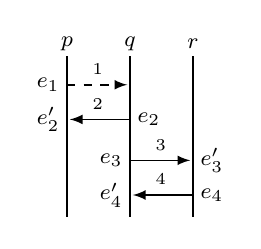
\begin{tikzpicture}[>=stealth,node distance=3.2cm,shorten >=1pt,
      every state/.style={text=black, scale =0.8}, semithick,
      font={\fontsize{8pt}{12}\selectfont}]
	\begin{scope}[xshift = 9cm, scale = 0.8]
		\node at (-0.3, -0.65)  (e)    {$e_1$};
		\node at (1.3, -1.2)  (e)    {$e_2$};
		\node at (-0.3, -1.2)  (e)    {$e_2'$};
		\node at (0.7, -1.85)  (e)    {$e_3$};
		\node at (2.3, -1.85)  (e)    {$e_3'$};
		\node at (2.3, -2.4)  (e)    {$e_4$};
		\node at (0.7, -2.4)  (e)    {$e_4'$};
		%MACHINES
		\draw (0,0) node{$p$} ;
		\draw (1,0) node{$q$} ;
		\draw (2,0) node{$r$} ;
		\draw (0,-0.2) -- (0,-2.8) ;
		\draw (1,-0.2) -- (1,-2.8);
		\draw (2, -0.2) -- (2, -2.8) ;
		%MESSAGES
		\draw[>=latex,->, dashed] (0,-0.65) -- (1, -0.65) node[midway,above]{$\amessage_1$};

		\draw[>=latex,->] (1, -1.2) -- (0, -1.2) node[midway, above] {$\amessage_2$};

		\draw[>=latex,->] (1,-1.85) -- (2,-1.85) node[midway, above] {$\amessage_3$};

		\draw[>=latex,->] (2,-2.4) -- (1,-2.4) node[midway,above] {$\amessage_4$};
	\end{scope}

\end{tikzpicture}
\captionof{figure}{MSC $\mscweakuniver$}
\label{fig:msc_weak_univer}
\end{center}
%\alain{NIce}
%\end{figure}

\end{minipage}

\paragraph*{Mailbox MSCs.}

For an MSC $\msc = (\Events,\procrel,\lhd,\lambda)$, we define
an additional binary relation that represents a constraint
under the mailbox semantics, where each process has only one incoming channel.
Let ${\mbrel}_\msc \subseteq \Events \times \Events$
be defined by: $e_1 \mbrel_\msc e_2$ if there is $q \in \Procs$
such that $\lambda(e_1) \in \qsAct{q}$,
$\lambda(e_2) \in \qsAct{q}$, and one of the following holds:
\begin{itemize}\itemsep=0.5ex
\item $e_1 \in \Matched{\msc}$ and $e_2 \in \Unm{\msc}$, or
\item $e_1 \lhd f_1$ and $e_2 \lhd f_2$ for some $f_1,f_2 \in \Events_q$ such that $f_1 \procrel^+ f_2$.
\end{itemize}

We let ${\preceq_\msc} = ({\procrel} \,\cup\, {\lhd} \,\cup\, {\mbrel_\msc})^\ast$.
Note that ${\le_\msc} \subseteq {\preceq_\msc}$.
%
%\begin{definition}\label{def:mailbox-msc}
We call $\msc \in \ppMSCs$ a \emph{mailbox MSC}
if ${\preceq_\msc}$ is a partial order.
%\end{definition}
Intuitively, this means that events can be scheduled in a way that corresponds
to the mailbox semantics, i.e., with one incoming channel per process.
Following the terminology in \cite{DBLP:conf/cav/BouajjaniEJQ18}, we also say that
a mailbox MSC satisfies \emph{causal delivery}.
The set of mailbox MSCs $\msc \in \ppMSCs$ is denoted by $\cdMSCs$.

\begin{example}\label{ex:mailbox-msc}
    MSC $\mscweakuniver$ is a mailbox MSC. Indeed, even though the order $\linrel$ defined in Example~\ref{ex:msc} does not respect all mailbox constraints, particularly the fact that $e_4 \mbrel_{\mscweakuniver} e_1$, there is a total order $ {\mblin} \supseteq {\preceq_{\mscweakuniver}}$ such that $
    e_2 \mblin e_3 \mblin e_3' \mblin e_4 \mblin e_1 \mblin e_2' \mblin e_4'$. We call $\mblin$ a mailbox linearization, which is formally defined below.
\end{example}

\paragraph*{Linearizations, Prefixes, and Concatenation.}

Consider $\msc = (\Events,\procrel,\lhd,\lambda) \in \MSCs$.
A \emph{\pp linearization} (or simply \emph{linearization}) of $\msc$ is a (reflexive) total order
${\linrel} \subseteq \Events \times \Events$ such that ${\le_\msc} \subseteq
{\linrel}$. Similarly,
a \emph{mailbox linearization} of $\msc$ is a total order
${\linrel} \subseteq \Events \times \Events$ such that ${\preceq_\msc} \subseteq
{\linrel}$. That is, every mailbox linearization is a \pp linearization,
but the converse is not necessarily true (Example~\ref{ex:mailbox-msc}).
Note that an MSC is a mailbox MSC iff it has at least one mailbox linearization.

\medskip

Let $\msc = (\Events,\procrel,\lhd,\lambda) \in \MSCs$ and consider
$E \subseteq \Events$ such that $E$ is ${\le_\msc}$-\emph{downward-closed}, i.e,
for all $(e,f) \in {\le_\msc}$ such that $f \in E$, we also have $e \in E$.
Then, the MSC $(E,{\procrel} \cap (E \times E),{\lhd} \cap (E \times E),\lambda')$,
where $\lambda'$ is the restriction of $\Events$ to $E$, is called a \emph{prefix}
of $\msc$. In particular, the empty MSC is a prefix of $\msc$.
We denote the set of prefixes of $\msc$ by $\Pref{\msc}$.
This is extended to sets $L \subseteq \MSCs$ as expected, letting
$\Pref{L} = \bigcup_{\msc \in L} \Pref{\msc}$.

\begin{lemma}
\label{lem:mb-prefix}
Every prefix of a mailbox MSC is a mailbox MSC.
\end{lemma}
\begin{proof}
Let $\msc = (\Events, \procrel, \lhd, \lambda) \in \mbMSCs$ and $\msc_0 =
(\Events_0, \procrel_0, \lhd_0, \lambda_0)$ be a prefix of $\msc$, i.e.,
$\Events_0 \subseteq \Events$. By contradiction, suppose that $\msc_0$ is not a
mailbox MSC. Then, there are distinct $e,f \in \Events_0$ such that $e \preceq_{M_0} f \preceq_{M_0}
e$ with ${\preceq_{\msc_0}} = ({\rightarrow_0} \cup {\lhd_0} \cup {\mbrel_{\msc_0}})^*$.
As $\Events_0 \subseteq \Events$, we have that ${\rightarrow_0} \subseteq {\rightarrow}$, ${\lhd_0} \subseteq {\lhd}$, and ${\mbrel_{\msc_0}} \subseteq {\mbrel_{\msc}}$. Finally, ${\preceq_{\msc_0}} \subseteq {\preceq_{\msc}}$ and $\msc$ is not a mailbox MSC, which is a contradiction.
\end{proof}

Let $\msc_1 = (\Events_1,\procrel_1,\lhd_1,\lambda_1)$ and
$\msc_2 = (\Events_2,\procrel_2,\lhd_2,\lambda_2)$ be two MSCs.
Their \emph{concatenation} $\msc_1 \cdot \msc_2 = (\Events,\procrel,\lhd,\lambda)$ is defined if, for all $(p,q) \in \Ch$,
$e_1 \in \Unm{\msc_1}$, and
$e_2 \in \Events_2$ such that $\lambda(e_1) \in \pqsAct{p}{q}$
and $\lambda(e_2) \in \pqsAct{p}{q}$,
we have $e_2 \in \Unm{\msc_2}$.
As expected, $\Events$ is the disjoint union of $\Events_1$ and $\Events_2$,
${\lhd}  = {\lhd_1} \cup {\lhd_2}$, $\lambda$ is the ``union'' of $\lambda_1$
and $\lambda_2$, and ${\procrel} = {\procrel_1} \cup {\procrel_2} \cup R$.
Here, $R$ contains, for all $p \in \Procs$ such that $(\Events_1)_p$ and
$(\Events_2)_p$ are non-empty, the pair $(e_1,e_2)$ where $e_1$ is the
maximal $p$-event in $M_1$ and $e_2$ is the minimal $p$-event in $M_2$.
Note that $\msc_1 \cdot \msc_2$ is indeed an MSC and that
concatenation is associative.

\subsection{Communicating Systems}

We now recall the definition of communicating systems (aka communicating finite-state
machines or message-passing automata), which consist of finite-state machines $A_p$
(one for every process $p \in \Procs$) that can communicate through the FIFO channels
from $\Ch$.

\begin{definition}\label{def:cs}
A \emph{communicating system} over $\Procs$ and $\Msg$ is a tuple
   $ \Sys = (A_p)_{p\in\procSet}$. For each
   $p \in \Procs$, $A_p = (Loc_p, \delta_p, \ell^0_p)$ is a finite transition system where
   $\Loc_p$ is a finite set of local (control) states, $\delta_p
   \subseteq \Loc_p \times \pAct{p} \times \Loc_p$ is the
   transition relation, and $\ell^0_p \in Loc_p$ is the initial state.
\end{definition}

Given $p \in \Procs$ and a transition $t = (\ell,a,\ell') \in \delta_p$, we let
$\tsource(t) = \ell$, $\ttarget(t) = \ell'$, $\tlabel(t) = a$, and
$\tmessage(t) = \msg$ if $a \in \msAct{\msg} \cup \mrAct{\msg}$.

\smallskip

There are in general two ways to define the semantics of a communicating system.
Most often it is defined as a global infinite transition system that keeps track
of the various local control states and all (unbounded) channel contents.
As, in this paper, our arguments are based on a graph view of MSCs, we will define
the language of $\Sys$ directly as a set of MSCs. These two semantic views are essentially
equivalent, but they have different advantages depending on the context.
We refer to \cite{CyriacG14} for a thorough discussion.

Let $\msc = (\Events,\procrel,\lhd,\lambda)$ be an MSC.
A \emph{run} of $\Sys$ on $\msc$ is a mapping
$\rho: \Events \to \bigcup_{p \in \Procs} \delta_p$
that assigns to every event $e$ the transition $\rho(e)$
that is executed at $e$. Thus, we require that
\begin{enumerate*}[label={(\roman*)}]
\item for all $e \in \Events$, we have $\tlabel(\rho(e)) = \lambda(e)$,
\item for all $(e,f) \in {\procrel}$, $\ttarget(\rho(e)) = \tsource(\rho(f))$,
\item for all $(e,f) \in {\lhd}$, $\tmessage(\rho(e)) = \tmessage(\rho(f))$,
and
\item for all $p \in \Procs$ and $e \in \Events_p$ such that there is no $f \in \Events$ with $f \procrel e$, we have $\tsource(\rho(e)) = \ell_p^0$.
\end{enumerate*}

Letting run $\Sys$ directly on MSCs is actually very convenient.
This allows us to associate with $\Sys$ its p2p language and mailbox language
in one go. The \emph{\pp language} of $\Sys$ is $\ppL{\Sys} = \{\msc \in \ppMSCs \mid$ there is a run of $\Sys$ on $\msc\}$.
The \emph{mailbox language} of $\Sys$ is $\mbL{\Sys} = \{\msc \in \mbMSCs \mid$ there is a run of $\Sys$ on $\msc\}$.

Note that, following \cite{DBLP:conf/cav/BouajjaniEJQ18,DBLP:conf/fossacs/GiustoLL20},
we do not consider final states or final configurations, as our purpose is to
reason about all possible
traces that can be \emph{generated} by $\Sys$.
%We will discuss this issue in more detail later in the paper. \todo{Do we still discuss this in the conference version or can we omit this sentence?}
The next lemma is obvious for the p2p semantics and follows from Lemma~\ref{lem:mb-prefix} for
	the mailbox semantics.

\begin{lemma}\label{lem:prefix-closed}
For all $\comsymb \in \{\ppsymb, \mbsymb\}$, $\cL{\Sys}$ is prefix-closed:
$\Pref{\cL{\Sys}} \subseteq \cL{\Sys}$.
\end{lemma}

\begin{example}
	Fig.~\ref{fig:system_weak_univer} depicts $\systemweakuniver = (A_p, A_q, A_r)$ such that MSC $\mscweakuniver$ in Fig.~\ref{fig:msc_weak_univer} belongs to $\ppL{\systemweakuniver}$ and to $\mbL{\systemweakuniver}$.
	There is a unique run $\rho$ of $\systemweakuniver$ on $\mscweakuniver$.
	We can see that $(e_3',e_4) \in {\rightarrow}$ and $\ttarget(\rho(e_3')) = \tsource(\rho(e_4)) = \ell_r^{1}$, $(e_2, e_2') \in \lhd_{\mscweakuniver}$, and $\tmessage(\rho(e_2)) = \tmessage(\rho(e_2')) = \msg_2$.
	\end{example}
	\begin{figure}[t]
	\begin{center}
	  \begin{tikzpicture}[>=stealth,node distance=3.2cm,shorten >=1pt,
		every state/.style={text=black, scale =0.75}, semithick,
		font={\fontsize{8pt}{12}\selectfont},
		scale = 0.9
		]
	  \begin{scope}[->]
		  \node[state,initial,initial text={}] (q0)  {$\ell_p^{0}$};
		  \node[state, right of=q0] (q1)  {$\ell_p^{1}$};
				\node[state, right of=q1] (q2) {$\ell_p^{2}$};
	
			\path (q0) edge node [above] {$\send{p}{q}{\msg_1}$} (q1);
				\path (q1) edge node [above] {$\rec{q}{p}{\msg_2}$}(q2);
			\node[thick] at (-1.1,0) {$A_p$};
	  \end{scope}
	
	  \begin{scope}[->, shift={(7.5,0)}]
		  \node[state,initial,initial text={}] (q0)  {$\ell_q^{0}$};
				\node[state, right of=q0] (q1)  {$\ell_q^{1}$};
				\node[state, below of=q1, node distance = 1.5cm] (q2) {$\ell_q^{2}$};
				\node[state, left of=q2] (q3)  {$\ell_q^{3}$};
	
				\path (q0) edge node [above] {$\send{q}{p}{\msg_2}$} (q1);
				\path (q1) edge node [right] {$\send{q}{r}{\msg_3}$}(q2);
				\path (q2) edge node [above] {$\rec{r}{q}{\msg_4}$} (q3);
				\node[thick] at (-1.1,0) {$A_q$};
	  \end{scope}
	
		\begin{scope}[->, shift={(0,-1.25)} ]
		  \node[state,initial,initial text={}] (q0)  {$\ell_r^{0}$};
				\node[state, right of=q0] (q1)  {$\ell_r^{1}$};
				\node[state, right of=q1] (q2) {$\ell_r^{2}$};
	
				\path (q0) edge node [above] {$\rec{q}{r}{\msg_3}$} (q1);
				\path (q1) edge node [above] {$\send{r}{q}{\msg_4}$}(q2);
				\node[thick] at (-1.1,0) {$A_r$};
	  \end{scope}
	\end{tikzpicture}
	\captionof{figure}{System $\systemweakuniver$}
	\label{fig:system_weak_univer}
	\end{center}
	\end{figure}	

\subsection{Conflict Graph}

We now recall the notion of a conflict graph associated to an MSC defined in \cite{DBLP:conf/cav/BouajjaniEJQ18}. This graph is used to depict the causal dependencies between message exchanges.  Intuitively, we have a dependency whenever
two messages have a process in common. For instance, an $\xrightarrow{SS}$
dependency between message exchanges $v$ and $v'$ expresses the fact that
$v'$ has been sent after $v$, by the same process. This notion is of interest because it was seen in \cite{DBLP:conf/cav/BouajjaniEJQ18} that the notion of synchronizability in MSCs (which is studied in this paper) can be graphically characterized by the nature of the associated conflict graph.
It is defined in terms of linearizations
in \cite{DBLP:conf/fossacs/GiustoLL20}, but we equivalently express it
directly in terms of MSCs.

\newcommand{\type}{\tau}
\newcommand{\stype}{S}
\newcommand{\rtype}{R}
\newcommand{\mexch}{\mu}
\newcommand{\Edges}{\mathit{Edges}}
\newcommand{\Nodes}{\mathit{Nodes}}

For an MSC $\msc = (\Events, \rightarrow, \lhd, \lambda)$ and
$e \in \Events$, we define the type $\type(e) \in \{\stype,\rtype\}$ of $e$ by $\type(e) = \stype$ if $e \in \SendEv{\msc}$
and $\type(e) = \rtype$ if $e \in \RecEv{\msc}$.
Moreover, for $e \in \Unm{\msc}$, we let $\mexch(e) = e$,
and for $(e,e') \in \lhd$, we let $\mexch(e) = \mexch(e') = (e,e')$.


\begin{definition}[Conflict graph]
	The \emph{conflict graph} $\cgraph{\msc}$ of an MSC $\msc = (\Events, \rightarrow, \lhd, \lambda)$ is the labeled graph $(\Nodes, \Edges)$, with $\Edges \subseteq \Nodes \times \{\stype,\rtype\}^2 \times \Nodes$, defined by
	$\Nodes = {\lhd} \cup \Unm{\msc}$ and $\Edges = \{(\mu(e),\type(e)\type(f),\mu(f)) \mid (e,f) \in {\to^+}\}$.
In particular, a node of $\cgraph{\msc}$ is either a single unmatched send event or a message pair $(e,e') \in {\lhd}$.
\end{definition}	

\subsection{Logic and Special Tree-Width}

\paragraph*{Monadic Second-Order Logic.}
The set of MSO formulas over MSCs (over $\Procs$ and $\Msg$) is given by the grammar
$
\phi ::= x \procrel y \mid x \lhd y \mid \lambda(x) = a \mid x = y \mid x \in X \mid \exists x.\phi \mid \exists X.\phi \mid \phi \vee \phi \mid \neg \phi
$,
where $a \in \Act$, $x$ and $y$ are first-order variables, interpreted as
events of an MSC, and $X$ is a second-order variable, interpreted
as a set of events. We assume that we have an infinite supply of variables,
and we use common abbreviations such as $\wedge$, $\forall$, etc.
The satisfaction relation is defined in the standard way and self-explanatory.
For example, the formula $\neg\exists x.(\bigvee_{a \in \sAct} \lambda(x) = a \;\wedge\; \neg \mathit{matched}(x))$
with $\mathit{matched}(x) = \exists y.x \lhd y$
says that there are no unmatched send events.
It is not satisfied by  MSC $\mscweakuniver$
of Fig.~\ref{fig:msc_weak_univer},
as message $\msg_1$ is not received,
but by $\mscstrongexist$ from Fig.~\ref{fig:msc_strong_exist}.

Given a sentence $\phi$, i.e., a formula without free variables,
we let $L(\phi)$ denote the set of (p2p) MSCs that satisfy $\phi$.
%
It is worth mentioning that the (reflexive) transitive closure of
a binary relation defined by an MSO formula with free variables $x$ and $y$,
such as $x \procrel y$, is MSO-definable so that the logic can freely
use formulas of the form $x \procrel^+ y$ or $x \le y$ (where $\le$
is interpreted as $\le_\msc$ for the given MSC $\msc$).
Therefore, the definition of a mailbox MSC can be readily translated into
the formula $\mbformula = \neg \exists x.\exists y.(\neg (x = y) \wedge x \preceq y \wedge y \preceq x)$ so that we have $L(\mbformula) = \mbMSCs$.
Here, $x \preceq y$ is obtained as the MSO-definable reflexive transitive closure of
the union of the MSO-definable relations $\procrel$, $\lhd$, and $\sqsubset$.
In particular, we may define $x \sqsubset y$ by :
\[
x \sqsubset y =
\displaystyle
\hspace{-1em}\bigvee_{\substack{q \in \Procs\\a,b \in \qsAct{q}}}\hspace{-1em}
\lambda(x) = a \;\wedge\; \lambda(y) = b
\wedge
\left(
\begin{array}{rl}
& \mathit{matched}(x) \wedge \neg \mathit{matched}(y)\\[1ex]
\vee & \exists x'.\exists y'. (x \lhd x' \;\wedge\; y \lhd y' \;\wedge\; x' \procrel^+ y')
\end{array}
\right)
\]

\paragraph*{Special Tree-Width.}

\emph{Special tree-width} \cite{Courcelle10},
is a graph measure that indicates how close
a graph is to a tree (we may also use classical
	\emph{tree-width} instead).
This or similar measures are commonly employed in verification. For instance, tree-width and split-width have been used in \cite{MadhusudanP11} and, respectively, \cite{DBLP:conf/concur/CyriacGK12,AiswaryaGK14} to reason about graph behaviors generated by pushdown and queue systems.
%Here we apply it to reason about MSCs.
There are several ways to define the special tree-width of an MSC.
We adopt the following game-based definition from \cite{DBLP:journals/corr/abs-1904-06942}.

Adam and Eve play a two-player turn based ``decomposition game''
whose positions
are MSCs with some pebbles placed on some events.
More precisely, Eve's positions are
\emph{marked MSC fragments} $(M, U)$, where
$\msc = (\Events, \procrel, \lhd, \lambda)$
is an \emph{MSC fragment} (an MSC with possibly some edges from
$\lhd$ or $\to$ removed)
 and $U \subseteq \Events$ is the subset of marked events.
Adam's positions are pairs of marked MSC fragments.
A move by Eve consists in the following steps:
\begin{enumerate}
	\item marking some events of the MSC resulting in $(M, U')$ with $U \subseteq U' \subseteq \Events$,
	\item removing (process and/or message) edges whose endpoints are marked,
	\item dividing $(M, U)$ in $(M_1, U_1)$ and $(M_2, U_2)$ such that $M$ is the disjoint (unconnected) union of $M_1$ and $M_2$
	and marked nodes are inherited.
\end{enumerate}
When it is Adam's turn, he simply chooses one of the two marked MSC fragments.
The initial position is $(\msc,\emptyset)$ where $M$ is the (complete) MSC at hand. A terminal position is any position belonging to Eve such that all events are marked.
%
For $k \in \N$, we say that the game is $k$-winning for Eve if she has a (positional) strategy that allows her,
starting in the initial position and independently of Adam's moves, to reach a terminal position such that, in every single position visited along the play, there are at most $k+1$ marked events.

\newcommand{\CS}[2]{\mathsf{CS}_{(#1,#2)}}
\newcommand{\MSO}[2]{\mathsf{MSO}_{(#1,#2)}}
\newcommand{\LCPDL}[2]{\mathsf{LCPDL}_{(#1,#2)}}
\newcommand{\MSCpm}[2]{\mathsf{MSC}_{(#1,#2)}}
\newcommand{\mbMSCpm}[2]{\mathsf{MSC}_{(#1,#2)}^{\mathsf{mb}}}


\begin{fact}[\cite{DBLP:journals/corr/abs-1904-06942}]
	The special tree-width of an MSC is the least $k$ such that
	the associated game is $k$-winning for Eve.
\end{fact}

The set of MSCs whose special tree-width is at most $k$ is denoted by $\stwMSCs{k}$.